% Created by tikzDevice version 0.10.1 on 2016-09-01 16:00:11
% !TEX encoding = UTF-8 Unicode
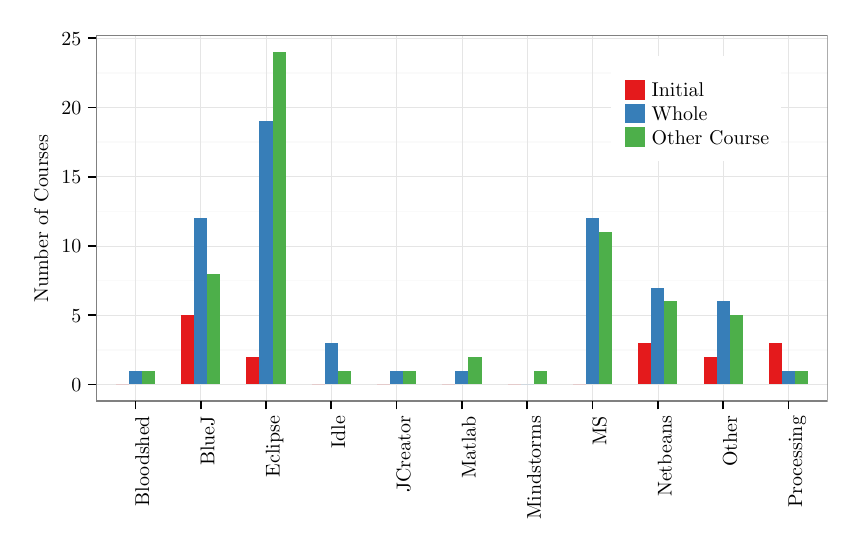
\begin{tikzpicture}[x=1pt,y=1pt]
\definecolor{fillColor}{RGB}{255,255,255}
\path[use as bounding box,fill=fillColor,fill opacity=0.00] (0,0) rectangle (289.08,180.67);
\begin{scope}
\path[clip] (  0.00,  0.00) rectangle (289.08,180.67);
\definecolor{drawColor}{RGB}{255,255,255}
\definecolor{fillColor}{RGB}{255,255,255}

\path[draw=drawColor,line width= 0.6pt,line join=round,line cap=round,fill=fillColor] (  0.00,  0.00) rectangle (289.08,180.68);
\end{scope}
\begin{scope}
\path[clip] ( 24.76, 45.74) rectangle (289.08,177.83);
\definecolor{fillColor}{RGB}{255,255,255}

\path[fill=fillColor] ( 24.76, 45.74) rectangle (289.08,177.83);
\definecolor{drawColor}{gray}{0.98}

\path[draw=drawColor,line width= 0.6pt,line join=round] ( 24.76, 64.25) --
	(289.08, 64.25);

\path[draw=drawColor,line width= 0.6pt,line join=round] ( 24.76, 89.27) --
	(289.08, 89.27);

\path[draw=drawColor,line width= 0.6pt,line join=round] ( 24.76,114.28) --
	(289.08,114.28);

\path[draw=drawColor,line width= 0.6pt,line join=round] ( 24.76,139.30) --
	(289.08,139.30);

\path[draw=drawColor,line width= 0.6pt,line join=round] ( 24.76,164.32) --
	(289.08,164.32);
\definecolor{drawColor}{gray}{0.90}

\path[draw=drawColor,line width= 0.2pt,line join=round] ( 24.76, 51.74) --
	(289.08, 51.74);

\path[draw=drawColor,line width= 0.2pt,line join=round] ( 24.76, 76.76) --
	(289.08, 76.76);

\path[draw=drawColor,line width= 0.2pt,line join=round] ( 24.76,101.78) --
	(289.08,101.78);

\path[draw=drawColor,line width= 0.2pt,line join=round] ( 24.76,126.79) --
	(289.08,126.79);

\path[draw=drawColor,line width= 0.2pt,line join=round] ( 24.76,151.81) --
	(289.08,151.81);

\path[draw=drawColor,line width= 0.2pt,line join=round] ( 24.76,176.83) --
	(289.08,176.83);

\path[draw=drawColor,line width= 0.2pt,line join=round] ( 38.92, 45.74) --
	( 38.92,177.83);

\path[draw=drawColor,line width= 0.2pt,line join=round] ( 62.52, 45.74) --
	( 62.52,177.83);

\path[draw=drawColor,line width= 0.2pt,line join=round] ( 86.12, 45.74) --
	( 86.12,177.83);

\path[draw=drawColor,line width= 0.2pt,line join=round] (109.72, 45.74) --
	(109.72,177.83);

\path[draw=drawColor,line width= 0.2pt,line join=round] (133.32, 45.74) --
	(133.32,177.83);

\path[draw=drawColor,line width= 0.2pt,line join=round] (156.92, 45.74) --
	(156.92,177.83);

\path[draw=drawColor,line width= 0.2pt,line join=round] (180.52, 45.74) --
	(180.52,177.83);

\path[draw=drawColor,line width= 0.2pt,line join=round] (204.12, 45.74) --
	(204.12,177.83);

\path[draw=drawColor,line width= 0.2pt,line join=round] (227.72, 45.74) --
	(227.72,177.83);

\path[draw=drawColor,line width= 0.2pt,line join=round] (251.32, 45.74) --
	(251.32,177.83);

\path[draw=drawColor,line width= 0.2pt,line join=round] (274.92, 45.74) --
	(274.92,177.83);
\definecolor{fillColor}{RGB}{228,26,28}

\path[fill=fillColor] ( 31.84, 51.74) rectangle ( 36.56, 51.74);
\definecolor{fillColor}{RGB}{55,126,184}

\path[fill=fillColor] ( 36.56, 51.74) rectangle ( 41.28, 56.74);
\definecolor{fillColor}{RGB}{77,175,74}

\path[fill=fillColor] ( 41.28, 51.74) rectangle ( 46.00, 56.74);
\definecolor{fillColor}{RGB}{228,26,28}

\path[fill=fillColor] ( 55.44, 51.74) rectangle ( 60.16, 76.76);
\definecolor{fillColor}{RGB}{55,126,184}

\path[fill=fillColor] ( 60.16, 51.74) rectangle ( 64.88,111.78);
\definecolor{fillColor}{RGB}{77,175,74}

\path[fill=fillColor] ( 64.88, 51.74) rectangle ( 69.60, 91.77);
\definecolor{fillColor}{RGB}{228,26,28}

\path[fill=fillColor] ( 79.04, 51.74) rectangle ( 83.76, 61.75);
\definecolor{fillColor}{RGB}{55,126,184}

\path[fill=fillColor] ( 83.76, 51.74) rectangle ( 88.48,146.81);
\definecolor{fillColor}{RGB}{77,175,74}

\path[fill=fillColor] ( 88.48, 51.74) rectangle ( 93.20,171.83);
\definecolor{fillColor}{RGB}{228,26,28}

\path[fill=fillColor] (102.64, 51.74) rectangle (107.36, 51.74);
\definecolor{fillColor}{RGB}{55,126,184}

\path[fill=fillColor] (107.36, 51.74) rectangle (112.08, 66.75);
\definecolor{fillColor}{RGB}{77,175,74}

\path[fill=fillColor] (112.08, 51.74) rectangle (116.80, 56.74);
\definecolor{fillColor}{RGB}{228,26,28}

\path[fill=fillColor] (126.24, 51.74) rectangle (130.96, 51.74);
\definecolor{fillColor}{RGB}{55,126,184}

\path[fill=fillColor] (130.96, 51.74) rectangle (135.68, 56.74);
\definecolor{fillColor}{RGB}{77,175,74}

\path[fill=fillColor] (135.68, 51.74) rectangle (140.40, 56.74);
\definecolor{fillColor}{RGB}{228,26,28}

\path[fill=fillColor] (149.84, 51.74) rectangle (154.56, 51.74);
\definecolor{fillColor}{RGB}{55,126,184}

\path[fill=fillColor] (154.56, 51.74) rectangle (159.28, 56.74);
\definecolor{fillColor}{RGB}{77,175,74}

\path[fill=fillColor] (159.28, 51.74) rectangle (164.00, 61.75);
\definecolor{fillColor}{RGB}{228,26,28}

\path[fill=fillColor] (173.44, 51.74) rectangle (178.16, 51.74);
\definecolor{fillColor}{RGB}{55,126,184}

\path[fill=fillColor] (178.16, 51.74) rectangle (182.88, 51.74);
\definecolor{fillColor}{RGB}{77,175,74}

\path[fill=fillColor] (182.88, 51.74) rectangle (187.60, 56.74);
\definecolor{fillColor}{RGB}{228,26,28}

\path[fill=fillColor] (197.04, 51.74) rectangle (201.76, 51.74);
\definecolor{fillColor}{RGB}{55,126,184}

\path[fill=fillColor] (201.76, 51.74) rectangle (206.48,111.78);
\definecolor{fillColor}{RGB}{77,175,74}

\path[fill=fillColor] (206.48, 51.74) rectangle (211.20,106.78);
\definecolor{fillColor}{RGB}{228,26,28}

\path[fill=fillColor] (220.64, 51.74) rectangle (225.36, 66.75);
\definecolor{fillColor}{RGB}{55,126,184}

\path[fill=fillColor] (225.36, 51.74) rectangle (230.08, 86.77);
\definecolor{fillColor}{RGB}{77,175,74}

\path[fill=fillColor] (230.08, 51.74) rectangle (234.80, 81.76);
\definecolor{fillColor}{RGB}{228,26,28}

\path[fill=fillColor] (244.24, 51.74) rectangle (248.96, 61.75);
\definecolor{fillColor}{RGB}{55,126,184}

\path[fill=fillColor] (248.96, 51.74) rectangle (253.68, 81.76);
\definecolor{fillColor}{RGB}{77,175,74}

\path[fill=fillColor] (253.68, 51.74) rectangle (258.40, 76.76);
\definecolor{fillColor}{RGB}{228,26,28}

\path[fill=fillColor] (267.84, 51.74) rectangle (272.56, 66.75);
\definecolor{fillColor}{RGB}{55,126,184}

\path[fill=fillColor] (272.56, 51.74) rectangle (277.28, 56.74);
\definecolor{fillColor}{RGB}{77,175,74}

\path[fill=fillColor] (277.28, 51.74) rectangle (282.00, 56.74);
\definecolor{drawColor}{gray}{0.50}

\path[draw=drawColor,line width= 0.6pt,line join=round,line cap=round] ( 24.76, 45.74) rectangle (289.08,177.83);
\end{scope}
\begin{scope}
\path[clip] (  0.00,  0.00) rectangle (289.08,180.67);
\definecolor{drawColor}{RGB}{0,0,0}

\node[text=drawColor,anchor=base east,inner sep=0pt, outer sep=0pt, scale=  0.72] at ( 19.36, 49.26) {0};

\node[text=drawColor,anchor=base east,inner sep=0pt, outer sep=0pt, scale=  0.72] at ( 19.36, 74.28) {5};

\node[text=drawColor,anchor=base east,inner sep=0pt, outer sep=0pt, scale=  0.72] at ( 19.36, 99.30) {10};

\node[text=drawColor,anchor=base east,inner sep=0pt, outer sep=0pt, scale=  0.72] at ( 19.36,124.31) {15};

\node[text=drawColor,anchor=base east,inner sep=0pt, outer sep=0pt, scale=  0.72] at ( 19.36,149.33) {20};

\node[text=drawColor,anchor=base east,inner sep=0pt, outer sep=0pt, scale=  0.72] at ( 19.36,174.35) {25};
\end{scope}
\begin{scope}
\path[clip] (  0.00,  0.00) rectangle (289.08,180.67);
\definecolor{drawColor}{RGB}{0,0,0}

\path[draw=drawColor,line width= 0.6pt,line join=round] ( 21.76, 51.74) --
	( 24.76, 51.74);

\path[draw=drawColor,line width= 0.6pt,line join=round] ( 21.76, 76.76) --
	( 24.76, 76.76);

\path[draw=drawColor,line width= 0.6pt,line join=round] ( 21.76,101.78) --
	( 24.76,101.78);

\path[draw=drawColor,line width= 0.6pt,line join=round] ( 21.76,126.79) --
	( 24.76,126.79);

\path[draw=drawColor,line width= 0.6pt,line join=round] ( 21.76,151.81) --
	( 24.76,151.81);

\path[draw=drawColor,line width= 0.6pt,line join=round] ( 21.76,176.83) --
	( 24.76,176.83);
\end{scope}
\begin{scope}
\path[clip] (  0.00,  0.00) rectangle (289.08,180.67);
\definecolor{drawColor}{RGB}{0,0,0}

\path[draw=drawColor,line width= 0.6pt,line join=round] ( 38.92, 42.74) --
	( 38.92, 45.74);

\path[draw=drawColor,line width= 0.6pt,line join=round] ( 62.52, 42.74) --
	( 62.52, 45.74);

\path[draw=drawColor,line width= 0.6pt,line join=round] ( 86.12, 42.74) --
	( 86.12, 45.74);

\path[draw=drawColor,line width= 0.6pt,line join=round] (109.72, 42.74) --
	(109.72, 45.74);

\path[draw=drawColor,line width= 0.6pt,line join=round] (133.32, 42.74) --
	(133.32, 45.74);

\path[draw=drawColor,line width= 0.6pt,line join=round] (156.92, 42.74) --
	(156.92, 45.74);

\path[draw=drawColor,line width= 0.6pt,line join=round] (180.52, 42.74) --
	(180.52, 45.74);

\path[draw=drawColor,line width= 0.6pt,line join=round] (204.12, 42.74) --
	(204.12, 45.74);

\path[draw=drawColor,line width= 0.6pt,line join=round] (227.72, 42.74) --
	(227.72, 45.74);

\path[draw=drawColor,line width= 0.6pt,line join=round] (251.32, 42.74) --
	(251.32, 45.74);

\path[draw=drawColor,line width= 0.6pt,line join=round] (274.92, 42.74) --
	(274.92, 45.74);
\end{scope}
\begin{scope}
\path[clip] (  0.00,  0.00) rectangle (289.08,180.67);
\definecolor{drawColor}{RGB}{0,0,0}

\node[text=drawColor,rotate= 90.00,anchor=base east,inner sep=0pt, outer sep=0pt, scale=  0.72] at ( 43.88, 40.34) {Bloodshed};

\node[text=drawColor,rotate= 90.00,anchor=base east,inner sep=0pt, outer sep=0pt, scale=  0.72] at ( 67.48, 40.34) {BlueJ};

\node[text=drawColor,rotate= 90.00,anchor=base east,inner sep=0pt, outer sep=0pt, scale=  0.72] at ( 91.08, 40.34) {Eclipse};

\node[text=drawColor,rotate= 90.00,anchor=base east,inner sep=0pt, outer sep=0pt, scale=  0.72] at (114.68, 40.34) {Idle};

\node[text=drawColor,rotate= 90.00,anchor=base east,inner sep=0pt, outer sep=0pt, scale=  0.72] at (138.28, 40.34) {JCreator};

\node[text=drawColor,rotate= 90.00,anchor=base east,inner sep=0pt, outer sep=0pt, scale=  0.72] at (161.88, 40.34) {Matlab};

\node[text=drawColor,rotate= 90.00,anchor=base east,inner sep=0pt, outer sep=0pt, scale=  0.72] at (185.48, 40.34) {Mindstorms};

\node[text=drawColor,rotate= 90.00,anchor=base east,inner sep=0pt, outer sep=0pt, scale=  0.72] at (209.08, 40.34) {MS};

\node[text=drawColor,rotate= 90.00,anchor=base east,inner sep=0pt, outer sep=0pt, scale=  0.72] at (232.68, 40.34) {Netbeans};

\node[text=drawColor,rotate= 90.00,anchor=base east,inner sep=0pt, outer sep=0pt, scale=  0.72] at (256.28, 40.34) {Other};

\node[text=drawColor,rotate= 90.00,anchor=base east,inner sep=0pt, outer sep=0pt, scale=  0.72] at (279.88, 40.34) {Processing};
\end{scope}
\begin{scope}
\path[clip] (  0.00,  0.00) rectangle (289.08,180.67);
\definecolor{drawColor}{RGB}{0,0,0}

\node[text=drawColor,rotate= 90.00,anchor=base,inner sep=0pt, outer sep=0pt, scale=  0.72] at (  7.36,111.78) {Number of Courses};
\end{scope}
\begin{scope}
\path[clip] (  0.00,  0.00) rectangle (289.08,180.67);
\definecolor{fillColor}{RGB}{255,255,255}

\path[fill=fillColor] (210.83,132.53) rectangle (272.18,170.29);
\end{scope}
\begin{scope}
\path[clip] (  0.00,  0.00) rectangle (289.08,180.67);
\definecolor{fillColor}{RGB}{228,26,28}

\path[fill=fillColor] (215.81,154.58) rectangle (222.92,161.70);
\end{scope}
\begin{scope}
\path[clip] (  0.00,  0.00) rectangle (289.08,180.67);
\definecolor{fillColor}{RGB}{55,126,184}

\path[fill=fillColor] (215.81,146.05) rectangle (222.92,153.16);
\end{scope}
\begin{scope}
\path[clip] (  0.00,  0.00) rectangle (289.08,180.67);
\definecolor{fillColor}{RGB}{77,175,74}

\path[fill=fillColor] (215.81,137.51) rectangle (222.92,144.63);
\end{scope}
\begin{scope}
\path[clip] (  0.00,  0.00) rectangle (289.08,180.67);
\definecolor{drawColor}{RGB}{0,0,0}

\node[text=drawColor,anchor=base west,inner sep=0pt, outer sep=0pt, scale=  0.72] at (225.44,155.66) {Initial};
\end{scope}
\begin{scope}
\path[clip] (  0.00,  0.00) rectangle (289.08,180.67);
\definecolor{drawColor}{RGB}{0,0,0}

\node[text=drawColor,anchor=base west,inner sep=0pt, outer sep=0pt, scale=  0.72] at (225.44,147.12) {Whole};
\end{scope}
\begin{scope}
\path[clip] (  0.00,  0.00) rectangle (289.08,180.67);
\definecolor{drawColor}{RGB}{0,0,0}

\node[text=drawColor,anchor=base west,inner sep=0pt, outer sep=0pt, scale=  0.72] at (225.44,138.59) {Other Course};
\end{scope}
\end{tikzpicture}
